\documentclass[main.tex]{subfiles} 
\begin{document}

\section*{Drøfting}
Når elever skal vurderes så kan dette gjøres på flere måter:
\begin{itemize}
\item Normalfordeling og fast poengsum : da blir vurderingsgrunnlaget \emph{de andre elevenes prestasjoner}. 
Dette blir også referert som relativ vurdering. Vurdering av en individ avhenger da av de andre
elevenes prestasjoner. Ved fast poengsum innebærer det at det er etter poeng oppnåelse elevene blir vurdert. 
Da vil karakterene avgjøres ut ifra hvor mye peongsum eleven har klart å oppnå. Her vil ofte vanskelig oppgaver
bli vektlagt mer enn enkelere oppgaver.
\item Individrelatert kriterier : da vurderes eleven utelukkende i forhold til sine egne forutsetninger
og tidligere prestasjoner. I grunnskolen skal vurderingen uten karakterer i hovedsak være 
individrelatert  (\citeNP[s. 25]{hell07}).
\item Målrelatert kriterier : kvalitetsstandarden blir da en didaktisk kontretisering av kompetansemål.
 I grunnskolen skal vurderingen med karakterer skje etter målrelaterte kriterier (\citeNP[s. 26]{hell07}).
\item Kompetansemål : da vurderes elevene utfra hvilket nivå eller trinn (i henhold til Bloom's taksonomi) 
                      de demonstrer i sin oppnåelse av kompetansemålene.
\end{itemize}
Jeg er nok enig i at bruken av individrelatert vurdering er en god vurderingsgrunnlag i situasjoner
der karakterer ikke brukes. Denne vurderingsformen oppfyller kriterier for god vurdering, siden den brukes til å 
fortelle eleven hvor hen befinner seg i sin faglig progresjon. Når lærer og elev sammen setter individuelle mål, både 
nærliggende og langsikte, da vil eleven gjennom et slikt vurderingsgrunnlag få konkete tilbakemeldinger og 
fremovermeldinger som fokuserer på nettopp elevens prestasjoner og målsettinger som hen har laget sammen med
læreren (\citeNP[s. 200]{olma15}). Det kan også være fordelsaktig å koble målsettingene til kompetansenivå eleven 
demonstrerer og jobbe mot høyre kompetansenivå. For eksempel diskutere er et høyt kompetansenivå, der eleven 
kan trekke sammnenhenger og redegjøre for sine tanker om en problemstilling. I motsetning er å beskrive et middels 
kompetansenivå (i Bloom's taksonomi).

Ved kartlegging av elevenes svakheter og styrker, er det passende å bruke individrelaterte kritier 
(\citeNP[s. 25]{hell07}) og koble inn kompetansemålene. Dette er passende å bruke når det vurderes uten karakter. 
Til en kartleggingsprøve så er det 
vanskelig å trekke inn individrelaterte kriterier med mindre lærer har godt kjennskap til eleven på forhånd. Jeg 
koblet dessverre ikke inn kompetansemålene heller, noe som det bør brukes mer av. Gjennom noen av mine samtaler 
med elever, oppdaget jeg fort at det var få som trakk forbindelsen mellom egen læring og koblingen til kompetansemålene. 
For undervisere regnes det som en god praksis at elevene er alltid bevisste om hvorfor de lærer det de lærer og hvor 
de er på vei. \citeA[s. 136]{klet13} beskriver en god undervisningsseksens der lærere klarer å balansere mellom 
tilegnelses-, utprøvings-, og konsolideringssituasjoner. Ifølge Klette har norske klasserom ensidige tendenser i bruken 
av varierte arbeidsmåter. Slik det kan ses fra figur \ref{fig:odeg10}, er det for eksempel lite 
konsolideringssituasjoner. Lærernes metalæringsaktiviteter regnes som særlig avgjørende for å sikre elevenes læring 
(\citeNP[s. 186]{klet13}). Å bruke dette som et fast organiserende prinsipp, blir derimot sjelden gjennomført 
(\citeNP[s. 26]{odeg10}). Dermed er det viktig å koble inn kompetansemålene og jobbe målrettet mot høyere
kompetansenivå. Dette vil fremme læing hos eleven og gi eleven en pekepinn på hvor hen må ta tak.
\begin{figure}[h!]
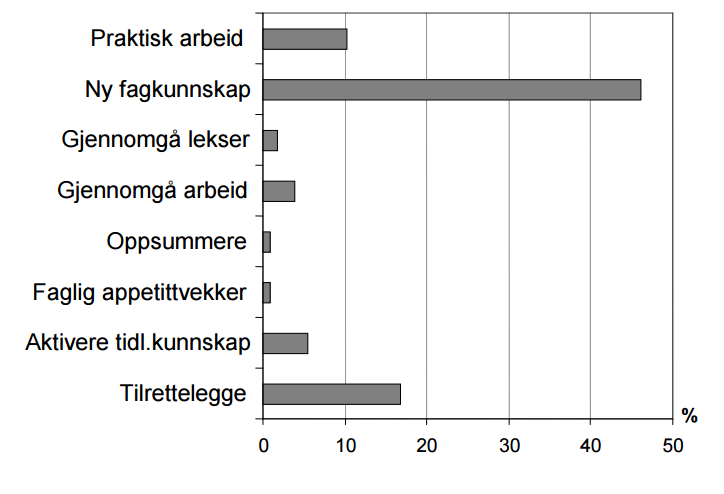
\includegraphics[scale = 0.6]{../figures/undervisnings_aktivitet.png}
\caption{Oversikt over naturfaglærernes undervisningstilbud til elevene fra PISA+ studie. Kilde: 
\protect\citeA{odeg10}.}
\label{fig:odeg10}
\end{figure}


Fra mine observasjoner og samtaler med elevene kom det frem at noen av 
elevene anstrengte ikke like hardt som de ellers ville ha gjort hvis kartleggingsprøven var en ``virkelig'' prøve.
Gjennom elevsamtale med en av de faglig sterke elevene, spurte jeg eleven hvorfor hen ikke hadde besvart en spesifikk 
oppgave og eleven svarte med å si at oppgaven var lett, men hen ``orket'' ikke å gå gjennom den. Grunnen hen oppga 
var at siden det ikke var en prøve, hadde det ikke så mye betydning. Dette samsvarer godt med det \citeA[s. 3]{brbl14} 
skriver : 
\begin{displayquote}
Vurdering kan ha en betydelig påvirkning på hvordan elever jobber, fordi de oppfatter det som 
vurderes som det eneste ``som teller''.
\end{displayquote}

Det er verdt å merke at hvis dette var 
en prøve så ville det ha vært viktig å skape situasjoner der elever kan vise mestring (\citeNP[s. 225]{abhk11}) (bruk 
flere kilder her). 

Lav fagelig selvtillit kan i en del tilfeller være et reelt hinder for å velge fysikk, spesielt blant jenter\citeNP[s. 225]{abhk11}.

Siden dette var en kartleggingsprøve var fokuset isteden rettet mot å avklare elevens misoppfattelser og få en oversikt 
over hvor elevene ligger i sin læringsprossess. Her vil jeg derfor påstå at det er viktig å gjøre et slikt skille, men 
det bør selvfølgelig skapes litt rom for å la elevene kjene på mestringsfølelsen. Dette vil jeg ta hensyn til videre i
mitt vurderingsarbeid. Videre nå vil jeg snakke om individuelle oppgaver fra kartleggingsprøven og diskutere 
elevenes feiltolninger.

\subsection*{Elevenes feiltolkninger}
Ifølge \citeA[s. 15]{brek02} og \citeA[s. 170]{olma15} kan diagnostiske oppgaver bli brukt til å identifisere og 
fremheve misoppfatninger som elevene har utviklet, gi læreren informasjon om elevenes løsningsstrategier og måle hvordan 
undervisningen har hjulpet elevene til å overvinne misoppfatningene. Gjennom blant annet kartleggingsprøver får elever 
muligheter til å utrykke sine skriftlige ferdigheter i naturfag. Å skrive i naturfag regnes som en av grunnleggende 
ferdighetene. Det innebærer blant å beskrive og forklare egen tankgegang. Skriving i naturfag blir sett på som et redskap for å utvikle egne tanker og egen læring (\citeNP{udirGF}). 

Dette er ofte misoppfattelser som også ligger hos elever ved ulike faglignivå. Gjennom praksis, i mitt forsøk med å 
rette disse misoppfattelser har vært å tydeliggjøre forskjellen mellom disse to reglene. 

\subsection*{Rom for tolkning blant elevenes misoppfattelser}

Dessverre er formuleringen ikke
godt nok til å trekke elevene inn i et diskurs. Her burde det gjerne ha blitt lagt til en bisetning, som 
for eksempel \emph{``Kan du gi en forklaring?''}. Med slike spørsmål er det lettere å oppdage elevenes
feiltolkninger, fordi da slipper en å få besvarelser som er enten ``ja'' eller ``nei''. 
Dette er en fin øvelse for elever å demonstrere at de har forstått bruken av X.


\subsection*{Tilbakemeldinger}

William redegjør for hvorfor tilbakemeldinger noen ganger kan føre til senking 
i elvenes ytelse. Han referer til Kluger og DeNisi (1996), når han summerer opp 
\begin{displayquote}
\textelp{} feedback was least effective when it focused on the task in hand, 
and more effective when it focused on the details at hand, and most effective 
when it focused on the details of the task and involved goal-setting.
(\citeNP[s. 140]{will10})
\end{displayquote}
For a vurderingsarbeidet
skal fremme læring hos eleven er det viktig at eleven kan delta i å sette egne
mål. Jeg kan tydeliggjøre disse målene for eleven gjennom fremovermeldinger,
men det er viktig for eleven å ha et forhold til disse målene.


\end{document}
